\begin{corrige}{devoir2-0009}
  \begin{enumerate}
  \item On voit sur le dessin que l'intersection entre les deux sphères $x^2+y^2+z^2=4$ et $x^2+y^2+(z-2)^2=4$ est un cercle. Pour trouver ses équations on passe d'abord en coordonnées sphériques :  $x^2+y^2+z^2=4$ devient $\rho=2$ et $x^2+y^2+(z-2)^2=4$ devient $\rho= 4\cos(\phi)$. L'intersection est donnée par le sicles de rayon $2$ et de $\phi= \arccos(1/2)= \pi/3$. La région dont on veut calculer le volume est alors donnée par $\phi\in[0, \pi/3]$, $\rho\in[2, 4\cos(\phi)] $ et $\theta \in [0, 2\pi]$. Le volume est donné par la valeur de l'intégrale suivante
    \begin{equation}
      \begin{aligned}
        \int_0^{2\pi}\int_0^{\pi/3}\int_2^{4\cos(\phi)}1 & \, \rho^2\sin(\phi)\, d\rho \, d\phi \, d\theta = 2\pi \int_0^{\pi/3}\frac{(4\cos(\phi))^3-2^3}{3} \sin(\phi)\, d\phi= \\
&= \frac{2\pi}{3}4^2\left( -\cos^4(\pi/3)+\cos^4(0)\right)+ \frac{2\pi}{3}2^3 \left( \cos(\pi/3)-\cos(0)\right)=\\
&=\frac{2\pi}{3}(-1+16 - 4) = \frac{22\pi}{3}.
      \end{aligned}
    \end{equation}

    \begin{figure}
      \begin{center}
        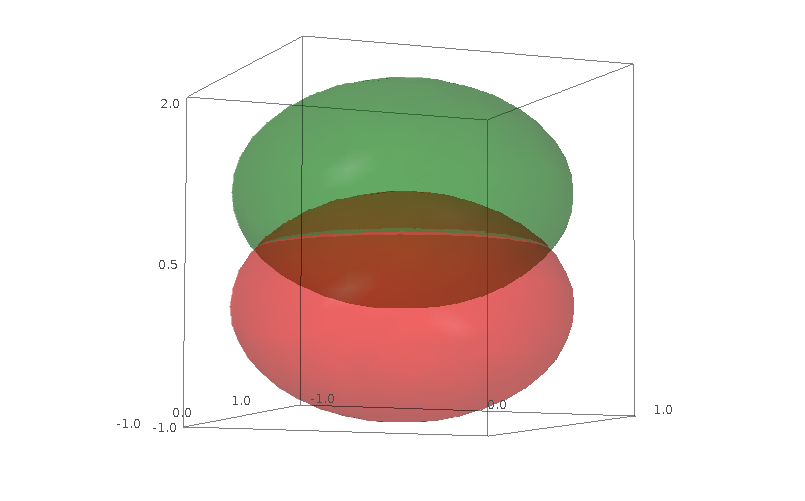
\includegraphics[width=8cm]{Fig_exo8devoir2.png}  
        \caption{Les deux sphères}\label{exo8devoir2}
      \end{center}
    \end{figure}
   
  \item Le domaine d'intégration $E$ est une pyramide renversée. Le rôle joué par les trois variables est symétrique. Les côtés de la pyramide sont des morceaux de droite entre les sommets $(0,0,0)$, $(0,0,2)$ $(0, 2, 2)$ et $(2, 0, 2)$. La pyramide est dont contenue dans le premier octant. 
 
On peut choisir librement  une variable de départ : ici je choisis $z$. On voit tout de suite que $z$ est dans l'intervalle $[0, 2]$. Ensuite, je considère $z$ fixée et je dois décrire le triangle qui est la section de la pyramide à la hauteur $z$. Les sommet de cet triangle sont donnés par $(0,0,z)$, $(0,z,z)$ et $(z,0,z)$. Encore une fois on peut choisir la variable qu'on on veut traiter en première. Je choisis $y$, elle parcourt l'intervalle $[0, z]$. Soient maintenant fixées $z$ et $y$ : la variable $x$ parcourt un petit morceau de droite entre $0$ et $z-y$. Maintenant nous écrivons l'intégrale : comme l'intervalle d'intégration pour $x$ dépend de $z$ et de $y$ il faut intégrer d'abord par rapport à $x$. Ensuite, comme $z$ apparaît dans la borne de $y$ il faut intégrer par rapport à $y$. La variable dont les bornes sont simplement des nombres réels est toujours la dernière.  

\begin{equation}
  \int_0^2\int_0^z\int_0^{z-y}x\, dx\,dy\,dz=\frac{1}{2}\int_0^2\int_0^z(z-y)^2\, dy \, dz = \frac{1}{6}\int_0^2 z^3 \,dz = \frac{1}{24} 16= \frac{2}{3}.
\end{equation}
  \end{enumerate}

  \begin{figure}
    \begin{center}
      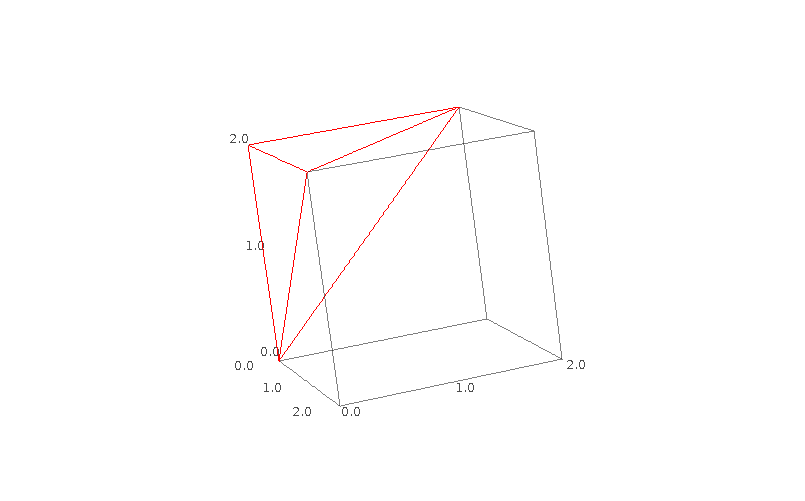
\includegraphics[width=9cm]{Fig_exo8devoir2deuxieme.png}
      
      \caption{Le domaine $E$}\label{exo8devoir2deuxieme}
    \end{center}
  \end{figure}
   
\end{corrige}
